%% \documentclass[sigplan,screen]{acmart}
%% \documentclass[sigplan,10pt,anonymous,review]{acmart}
\documentclass[sigplan,10pt,review]{acmart}
\settopmatter{printfolios=true,printccs=true,printacmref=false}

%%
%% \BibTeX command to typeset BibTeX logo in the docs
\AtBeginDocument{%
  \providecommand\BibTeX{{%
    \normalfont B\kern-0.5em{\scshape i\kern-0.25em b}\kern-0.8em\TeX}}}

%% Rights management information.  This information is sent to you
%% when you complete the rights form.  These commands have SAMPLE
%% values in them; it is your responsibility as an author to replace
%% the commands and values with those provided to you when you
%% complete the rights form.
\setcopyright{acmcopyright}
\copyrightyear{2020}
\acmYear{2020}
\acmDOI{10.1145/XXX}

%% These commands are for a PROCEEDINGS abstract or paper.
\acmConference[Woodstock '18]{Woodstock '18: ACM Symposium on Neural
  Gaze Detection}{June 03--05, 2018}{Woodstock, NY}
\acmBooktitle{Woodstock '18: ACM Symposium on Neural Gaze Detection,
  June 03--05, 2018, Woodstock, NY}
\acmPrice{15.00}
\acmISBN{978-1-4503-XXXX-X/18/06}


%% The majority of ACM publications use numbered citations and
%% references.  The command \citestyle{authoryear} switches to the
%% "author year" style.
%%
%% If you are preparing content for an event
%% sponsored by ACM SIGGRAPH, you must use the "author year" style of
%% citations and references.
%% Uncommenting
%% the next command will enable that style.
%%\citestyle{acmauthoryear}

%%%%%%%%%%%%%%%%%%%%%%%%%%%%%%%%%%%%%%%%%%%%%%%%%%%%%%%%%%%%%%%%%%%%%%%%%%%%%%%%

%% figure out which of these are actually used...
\usepackage{microtype}
\usepackage{mdframed}
\usepackage{colortab}
\usepackage{mathpartir}
\usepackage{bbm}
\usepackage{stmaryrd}
\usepackage{mathtools}
\usepackage{leftidx}
\usepackage{todonotes}
\usepackage{xspace}
\usepackage{wrapfig}
\usepackage{float}

\usepackage{amssymb}% http://ctan.org/pkg/amssymb
\usepackage{pifont}% http://ctan.org/pkg/pifont
\newcommand{\cmark}{\ding{51}}%
\newcommand{\xmark}{\ding{55}}%

% https://tex.stackexchange.com/questions/8549/how-can-i-draw-a-horizontal-line-spanning-only-some-of-the-table-cells
\usepackage{multirow}

\usepackage{enumitem}
\setlist
  { leftmargin = 5.5mm
  , itemsep = 3pt
  , topsep = 4pt
  }

\usepackage{alltt} %% temporary

% !TEX root = main.tex

\newcommand{\mynote}[3]{\textcolor{#3}{\textsf{{#2}}}}
\newcommand{\rkc}[1]{\mynote{rkc}{#1}{blue}}
\newcommand{\nick}[1]{\mynote{cy}{#1}{purple}}

\newcommand{\cvert}{{\,{\vert}\,}}

%% https://tex.stackexchange.com/questions/9796/how-to-add-todo-notes
\newcommand{\rkcTodo}[1]{\todo[linecolor=blue,backgroundcolor=blue!25,bordercolor=blue]{#1}}

\newcommand{\mattTodo}[1]{\todo[linecolor=green,backgroundcolor=green!2,bordercolor=green]{\tiny\textit{#1}}}
\newcommand{\mattOmit}[1]{\colorbox{yellow}{(Matt omitted stuff here)}}

\def\parahead#1{\paragraph{\textbf{#1.}}}
%% \def\paraheadNoDot#1{\paragraph{{\textbf{#1}}}}
\def\subparahead#1{\paragraph{\textit{#1.}}}
%% \def\paraheadindent#1{\paragraph{}\textit{#1.}}
%% \def\paraheadindentnodot#1{\paragraph{}\textit{#1}}

\newcommand{\ie}{i.e.}
\newcommand{\eg}{e.g.}
% \newcommand{\etc}{{\emph{etc.}}}
% \newcommand{\cf}{{\emph{cf.}}}
% \newcommand{\etal}{{\emph{et al.}}}

%% \newcommand{\hazel}{\ensuremath{\textsc{Hazel}}}
%% \newcommand{\sns}{\ensuremath{\textsc{Sketch-n-Sketch}}}
%% \newcommand{\deuce}{\ensuremath{\textsc{Deuce}}}
\newcommand{\Elm}{\ensuremath{\textsf{Elm}}}
\newcommand{\sns}{\ensuremath{\textrm{Sketch-n-Sketch}}}
\newcommand{\deuce}{\ensuremath{\textrm{Deuce}}}

\newcommand{\sectionDescription}[1]{\section{#1}}
\newcommand{\subsectionDescription}[1]{\subsection{#1}}
\newcommand{\subsubsectionDescription}[1]{\subsubsection{#1}}
%% \newcommand{\subsectionDescription}[1]{\subsection*{#1}}
\newcommand{\suppMaterials}{the Supplementary Materials}

\newcommand{\defeq}{\overset{\textrm{def}}{=}}

\newcommand{\eap}{action suggestion panel\xspace}
\newcommand{\Eap}{Action suggestion panel\xspace}

\newcommand{\myfootnote}[1]{\footnote{ #1}}

\def\sectionautorefname{Section}
\def\subsectionautorefname{Section}
\def\subsubsectionautorefname{Section}

\newcommand{\code}[1]{\lstinline{#1}}
\newcommand{\str}[1]
  {``#1''}

% Make italic?
%\newcommand{\Property}[1]{\emph{#1}}
\newcommand{\Property}[1]{\textrm{#1}}

% Calling out Cyrus's favorite verb, 'to be' ;)
\newcommand{\IS}{\colorbox{red}{is}\xspace}

\newcommand{\codeSize}
  %% {\footnotesize}
  {\small}

%\newcommand{\JoinTypes}[2]{\textsf{join}~~#1~~#2}
\newcommand{\JoinTypes}[2]{\textsf{join}(#1,#2)}

%% \newtheorem{theorem}{Theorem}[section] % 2.1, 2.2, etc.
\newtheorem{theorem}{Theorem}             % 1, 2, etc.
\newtheorem{remark}[theorem]{Remark}

%%%%%%%%%%%%%%%%%%%%%%%%%%%%%%%%%%%%%%%%%%%%%%%%%%%%%%%%%%%%%%%%%%%%%%%%%%%%%%%%
%% Spacing

\newcommand{\sep}{\hspace{0.06in}}
\newcommand{\sepPremise}{\hspace{0.20in}}
\newcommand{\hsepRule}{\hspace{0.20in}}
\newcommand{\vsepRuleHeight}{0.08in}
\newcommand{\vsepRule}{\vspace{\vsepRuleHeight}}
\newcommand{\miniSepOne}{\hspace{0.01in}}
\newcommand{\miniSepTwo}{\hspace{0.02in}}
\newcommand{\miniSepThree}{\hspace{0.03in}}
\newcommand{\miniSepFour}{\hspace{0.04in}}
\newcommand{\miniSepFive}{\hspace{0.05in}}
\newcommand{\breakAndIndent}
  {\mbox{}

   %% \hspace{0.15in}
   \hspace{0.00in}
  }

\newcommand{\justIndent}
  %% {\hspace{0.15in}
  {\hspace{0.00in}
  }

%%%%%%%%%%%%%%%%%%%%%%%%%%%%%%%%%%%%%%%%%%%%%%%%%%%%%%%%%%%%%%%%%%%%%%%%%%%%%%%%

% \lstset{
% %mathescape=true,basicstyle=\fontsize{8}{9}\ttfamily,
% literate={=>}{$\Rightarrow$}2
%          {<=}{$\leq$}2
%          {->}{${\rightarrow}$}1
%          {\\\\=}{\color{red}{$\lambda$}}2
%          {\\\\}{$\lambda$}2
%          {**}{$\times$}2
%          {*.}{${\color{blue}{\texttt{*.}}}$}2
%          {+.}{${\color{blue}{\texttt{+.}}}$}2
%          {<}{${\color{green}{\lhd}}$}1
%          {>?}{${\color{green}{\rhd}}$?}2
%          {<<}{${\color{green}{\blacktriangleleft}}$}1
%          {>>?}{${\color{green}{\blacktriangleright}}$?}2
%          {\{}{${\color{blue}{\{}}$}1
%          {\}}{${\color{blue}{\}}}$}1
%          {[}{${\color{purple}{[}}$}1
%          {]}{${\color{purple}{]}}$}1
%          {(}{${\color{darkgray}{\texttt{(}}}$}1
%          {)}{${\color{darkgray}{\texttt{)}}}$}1
%          {]]}{${\color{gray}{\big(}}$}1
%          {]]}{${\color{gray}{\big)}}$}1
% }

%%%%%%%%%%%%%%%%%%%%%%%%%%%%%%%%%%%%%%%%%%%%%%%%%%%%%%%%%%%%%%%%%%%%%%%%%%%%%%%%

\newcommand{\li}[1]{\lstinline[basicstyle=\ttfamily\fontsize{9pt}{1em}\selectfont]{#1}}
\newcommand{\lismall}[1]{\lstinline[basicstyle=\ttfamily\fontsize{9pt}{1em}\selectfont]{#1}}
\newcommand{\mapP}{\{0 \rightarrow \text{"a"}, 1 \rightarrow \text{"b"}, 3 \rightarrow \text{"c"}, 6 \rightarrow \text{"d"}, 10 \rightarrow \text{"e"}\}}
\newcommand{\dictP}{[(0, "a"), (0, "b"), (1, "c"), (2, "d"), (3, "e")]}

%%%%%%%%%%%%%%%%%%%%%%%%%%%%%%%%%%%%%%%%%%%%%%%%%%%%%%%%%%%%%%%%%%%%%%%%%%%%%%%%

%% \newcommand{\sal}{simple association list}
\newcommand{\sal}{association list}
\newcommand{\Sal}{Association List}
\newcommand{\SAL}{AL}

%% \newcommand{\cal}{canonicalized association list}
\newcommand{\cal}{canonical association list}
\newcommand{\Cal}{Canonical Association List}
\newcommand{\CAL}{CAL}
\newcommand{\Cals}{Canonical association lists}

%% \newcommand{\fpf}{finite partial function}
\newcommand{\fpf}{partial function}
\newcommand{\Fpf}{Partial Function}
\newcommand{\Fpfs}{Partial functions}
\newcommand{\FPF}{PF}

%% trying this out...
%% \newcommand{\cfpf}{canon. finite partial function}
\newcommand{\fpfk}{partial function with keys}
\newcommand{\Fpfk}{Partial Function with Keys}
\newcommand{\FPFK}{PFK}

\newcommand{\dd}{delta dictionary}
\newcommand{\dds}{delta dictionaries}
\newcommand{\Dd}{Delta Dictionary}
\newcommand{\Ddls}{Delta dictionaries}
\newcommand{\DD}{DD}

%%%%%%%%%%%%%%%%%%%%%%%%%%%%%%%%%%%%%%%%%%%%%%%%%%%%%%%%%%%%%%%%%%%%%%%%%%%%%%%%

\newcommand{\SemTot}{Semantic Totality}
%% \newcommand{\SemInj}{Semantic Injectivity}
\newcommand{\SemInj}{Extensionality}
\newcommand{\EqDec}{Decidable Equality}
%% \newcommand{\EzDstr}{Ease of Destruction}
\newcommand{\EzDstr}{Easy Destructibility}

%% tweak and remove indirection macros later, once terminology settles
\newcommand{\Total}{\SemTot}
\newcommand{\Extensional}{\SemInj}
\newcommand{\DecidableEq}{\EqDec}
\newcommand{\Destructible}{\EzDstr}

\newcommand{\total}{Total}
\newcommand{\extensional}{Extensional}
\newcommand{\decidable}{Decid. Eq.}
\newcommand{\destructible}{Destructible}

%%%%%%%%%%%%%%%%%%%%%%%%%%%%%%%%%%%%%%%%%%%%%%%%%%%%%%%%%%%%%%%%%%%%%%%%%%%%%%%%

% for use in alltt
\newcommand{\altFAll}{\ensuremath{\forall}}
\newcommand{\altRArr}{\ensuremath{\rightarrow}}
\newcommand{\altRARR}{\ensuremath{\Rightarrow}}
\newcommand{\altVdash}{\ensuremath{\vdash}}
\newcommand{\altAnd}{\ensuremath{\land}}
\newcommand{\altOr}{\ensuremath{\lor}}
\newcommand{\altNE}{\ensuremath{\ne}}
\newcommand{\altEmpty}{\ensuremath{\varnothing}}
\newcommand{\altIn}{\ensuremath{\in}}
\newcommand{\altNIn}{\ensuremath{\notin}}
\newcommand{\altSum}{\ensuremath{\sum}}
\newcommand{\altLAng}{\ensuremath{\langle}}
\newcommand{\altRAng}{\ensuremath{\rangle}}
\newcommand{\altLamb}{\ensuremath{\lambda}}
\newcommand{\altGam}{\ensuremath{\Gamma}}
\newcommand{\altCirc}{\ensuremath{\circ}}
\newcommand{\altCdot}{\ensuremath{\cdot}}


%%%%%%%%%%%%%%%%%%%%%%%%%%%%%%%%%%%%%%%%%%%%%%%%%%%%%%%%%%%%%%%%%%%%%%%%%%%%%%%%

\begin{document}

%%
%% The "title" command has an optional parameter,
%% allowing the author to define a "short title" to be used in page headers.

%% \title{Delta Dictionaries, or how to Cater Data Structures to Proof Assistants}

%% \title
%%   [Delta Dictionaries] %% : Unique Key-Value Associations in Proof Assistants]
%%   {Delta Dictionaries:\\Unique Key-Value Associations in Proof Assistants}

\title{Delta Dictionaries}
%% \subtitle{\total, \extensional, and \destructible{} Finite Maps in Proof Assistants}
\subtitle{\total{} and \extensional{} Finite Maps in Proof Assistants}

%%
%% The "author" command and its associated commands are used to define
%% the authors and their affiliations.
%% Of note is the shared affiliation of the first two authors, and the
%% "authornote" and "authornotemark" commands
%% used to denote shared contribution to the research.
\author{Anonymous}
\affiliation{%
  \institution{Anonymous}
}
\email{anonymous}
%% \orcid{1234-5678-9012}

%% \renewcommand{\shortauthors}{Trovato and Tobin, et al.}

\begin{teaserfigure}
\centering
%% \begin{figure*}
\newcommand{\lameq}[1]{$\lambda x$. $x = {#1}$}
\begin{tabular}{ l l }
 %% \Sal{} (\SAL) & [(3, "c"), (1, "b"), {\color{gray} (3, "q")}, (6, "d")] \\
 \Sal{} & [(3, "c"), (1, "b"), {\color{gray} (3, "q")}, (6, "d")] \\
 \Cal{} & [(1, "b"), (3, "c"), (6, "d")] \\ %% \quad (insert function dedupes and preserves canonical order)
 \Fpf{} & \lameq{3} ? "c" : (\lameq{1} ? "b" : (\lameq{3} ? {\color{gray} "q"} : (\lameq{6} ? "d" : $\bot$) $x$) $x$) $x$ \\
 %% \Fpfk{} & ((\lameq{3} ? "c" : (\lameq{1} ? "b" : (\lameq{3} ? {\color{gray} "q"} : (\lameq{6} ? "d" : $\bot$) $x$) $x$) $x$), [1, 3, 6])  \\
 \Dd{}  & [(1, "b"), (1, "c"), (2, "d")]
\end{tabular}
%% \caption{Dictionary representations which result from adding the sequence of keys 6, 3, 1, and 3 (again).}
%
%% \captionsetup{justification=centering}
%% \caption{Dictionary representations after mapping the sequence of keys 6, 3, 1, and 3 (again). \\
%% Each represents the same finite map: %% TODO macros if/when this stabilizes
%% \{ $1 \mapsto ``b"$, $3 \mapsto ``c"$, $6 \mapsto ``d"$ \}
%% }
%
\caption{Dictionary representations after inserting the sequence of keys 6, 3, 1, and 3:
\{ $1 \mapsto ``b"$, $3 \mapsto ``c"$, $6 \mapsto ``d"$ \}
}
%
\label{fig:intro-example}
%% \end{figure*}
\vspace{0.15in} %% SPACE HACK: between teaser figure and Abstract
%% \vspace{0.05in} %% SPACE HACK: between teaser figure and Abstract
\end{teaserfigure}


% !TEX root = ?.tex

%% no citations in Abstract
%%
%% \cite{?}

\begin{abstract}
Dictionaries (a.k.a. finite maps) are a core tool in any programming environment.
Conventional languages implement dictionaries with hashtables or auto-balanced trees, but proof assistants
- which favor simplicity and provability over performance - generally use association lists
(with or without canonical ordering) or finite partial functions. These solutions are suitable for many
cases - however, each one has a drawback: unordered lists can contain duplicates or have arbitrary ordering,
canonically ordered lists may be invalid and so must be refined with a proof of validity, and equality of finite partial
functions is undecidable. Using a variant of delta-encoding, we develop a novel list-based solution that preserves
canonical ordering while ensuring that every type-correct list is semantically valid, eliminating the need for refinement
with a proof of validity. Our solution also establishes a one-to-one correspondence between dictionary terms and semantic
mappings. We demonstrate the practical importance of these properties when developing metatheory for environment-based
evaluation semantics, while acknowledging that drawbacks of our solution may make it inferior to one of the conventional
solutions in some cases where that conventional solution is viable. We prove the relevant metatheory in Agda.
%
% Our solution is not suitable for all key types, and is harder to destruct or
%iterate than other list-of-pair solutions, but is nonetheless better suited to many large, complex program
%foundations metatheories than the existing solutions.
%
% Although easy to define and reason about, this approach has the disadvantage that keys
%can be duplicated, leading to the fact that many distinct lists represent the same semantic mapping.
%This many-one relationship creates various difficulties when used in practice, such as when proving
%contraction and exchange for a type-checking judgment.
\end{abstract}


%%
%% The code below is generated by the tool at http://dl.acm.org/ccs.cfm.
%% Please copy and paste the code instead of the example below.
%%
\begin{CCSXML}
<ccs2012>
   <concept>
       <concept_id>10011007.10010940.10010992.10010998.10010999</concept_id>
       <concept_desc>Software and its engineering~Software verification</concept_desc>
       <concept_significance>300</concept_significance>
       </concept>
   <concept>
       <concept_id>10011007.10011006</concept_id>
       <concept_desc>Software and its engineering~Software notations and
tools</concept_desc>
       <concept_significance>300</concept_significance>
       </concept>
   <concept>
       <concept_id>10003752.10003790.10002990</concept_id>
       <concept_desc>Theory of computation~Logic and verification</concept_desc>
       <concept_significance>300</concept_significance>
       </concept>
 </ccs2012>
\end{CCSXML}

\ccsdesc[300]{Software and its engineering~Software verification}
\ccsdesc[300]{Software and its engineering~Software notations and tools}
\ccsdesc[300]{Theory of computation~Logic and verification}

%%
%% Keywords. The author(s) should pick words that accurately describe
%% the work being presented. Separate the keywords with commas.
\keywords{proof assistants, data structures, dictionaries, Agda}

\maketitle

\section{Introduction}
\label{sec:Introduction}

%%%%%%%%%%%%%%%%%%%%%%%%%%%%%%%%%%%%%%%%%%%%%%%%%%%%%%%%%%%%%%%%%%%%%%%%%%%%%%%%
%% \rkc{Part 1.1: Motivation and SAL/CAL/FPF. Editing TBD.}

Conventionally, the design of data structures and algorithms is chiefly focused on performance, which is of significantly diminished concern in proof assistants.
%
As such, proof assistants often use entirely different data structures than those of conventional settings, with a focus on simplicity or useful proof-theoretic properties.

Consider dictionaries, which---among a broad range of purposes---are often used for implementing type contexts and evaluation environments.
%
The most basic representation for a dictionary, an \emph{\sal}, comprises a list of key-value pairs~\citep[Lists]{Pierce:SF1}.
%
Association lists are simple to create, manipulate, and reason about.
%
But because they allow duplicate bindings for the same key and they are sensitive to the order of insertions, many distinct \sal{}s represent the same semantic mapping.
%
For example, first two lines of \autoref{fig:intro-example}
%
%% ---and illustrated below in \autoref{fig:uneq}---
%
show two distinct association lists (among others) to represent a dictionary with three particular bindings.
%
This lack of \emph{\Extensional} can make proofs more difficult~\cite[Maps]{Pierce:SF1} or impossible, esp. when it comes to proving \emph{contraction} and \emph{exchange}%
\citep{StructProp}
%
(discussed further in \autoref{sec:Discussion:Generality}).

%% %% \begin{figure}[b]
\begin{figure}[h]
  \centering
  \begin{tikzpicture}[nodes = {align = left}]
    %% \node [scale=.45]
    \node [scale=.33]
    {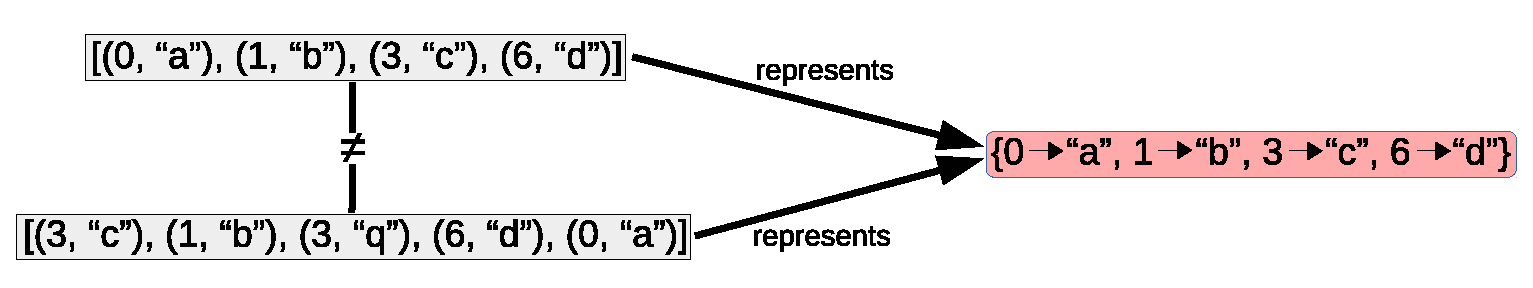
\includegraphics{figs/unequal.eps}};
  \end{tikzpicture}
  \caption{Two distinct \sal{}s representing the same semantic mapping. \rkc{Let's show the first two rows from Fig 1. And let's fit this into one column.}}
  \label{fig:uneq}
\end{figure}


\newcommand{\no}
  %% {No}
  %% {}
  {\color{lightgray}\phantom{$^*$}\xmark\phantom{$^*$}}
\newcommand{\noIO}
  %% {\color{lightgray}\phantom{$^*$}\xmark$^*$}
  {{\color{lightgray}\phantom{$^*$}\xmark}\footnotemark[3]} % 3 is hard-coded, but I see no other way
\newcommand{\yes}
  %% {Yes}
  %% {\phantom{*}\cmark\phantom{*}}
  {\phantom{$^-$}\cmark\phantom{$^-$}}
\newcommand{\yesMinus}
  %% {Yes*}
  %% {\phantom{*}\cmark*}
  {\phantom{$^-$}\cmark$^-$}
\newcommand{\yesPlus}
  %% {Yes*}
  %% {\phantom{*}\cmark*}
  {\phantom{$^-$}\cmark$^+$}
\newcommand{\eq}
  %% {Decidable equality}
  %% {Eq K}
  %% {(=) : (K,K) -> Bool}
  {$(=)$}
\newcommand{\ord}
  %% {Orderable}
  %% {Eq K, Ord K}
  %% {(=),(<) : (K,K) -> Bool}
  {$(=), (<)$}
\newcommand{\isoNat}
  %% {Bijects to naturals}
  %% {K $\leftrightarrow$ Nat}
  {$f\hspace{0.02in}\!:\!\hspace{0.02in}K \leftrightarrow \textit{Nat}$}

\newcommand{\header}[1]
  {\makebox[0.67in]{#1}}
\newcommand{\headers}[6]
  {&\header{#1}&\header{#2}&\header{#3}&\header{#4}&\header{#5}&\header{#6}}

%% \begin{figure}[H]
\begin{figure*}[t]
  \begin{tabular}{ l || c | c | c | c | c || c}
  \multirow{2}{*}{}
           & \multicolumn{5}{c||}{\footnotesize Client Usage}
           & {\footnotesize Implementation} \\ \cline{2-7}
   \headers{\total}{\extensional}{\decidable}{\destructible}{Key Type $K$}{Simple}    \\ \hline
   \Sal    & \yes   & \no        & \yes      & \yes         & \eq       & \yesPlus  \\ %% \hline
   \Cal    & \no    & \yes       & \yes      & \yes         & \ord      & \yesMinus \\ %% \hline
   \Fpf    & \noIO  & \yes       & \no       & \no          & \eq       & \yes      \\ \hline
   %% \Fpfk   & \no    & \yes       & \yes      & \yes         & \ord      & \simple     \\ \hline
   \Dd     & \yes   & \yes       & \yes      & \yesMinus    & \isoNat   & \no
  \end{tabular}
  \caption{Properties of dictionary representations.}
  \label{fig:prop-summary}
\end{figure*}
%% \end{figure}
 %% here to force layout on p.2

To establish a one-to-one correspondence between association lists and semantic mappings, one solution~\citep{FMapList} is to maintain a \emph{canonical}
%
form that is semantically valid and unique, namely, a list in which there are no duplicate keys and, furthermore, where keys are in sorted order.%
%
\footnote{\hspace{0.01in}%
%
Some treatments, including the Coq standard library~\citep{FMapInterface}, describe unordered but deduplicated \sal{}s as ``weak,'' implying that \cal{}s are ``strong.''
%
}
%
The second association list described in \autoref{fig:intro-example} is one such example.
%
This approach is \emph{\extensional} -- \ie{} it permits using built-in equality for semantic equivalence. However, it requires extending the underlying list type---which allows arbitrary, possibly invalid lists---with a proof of validity that refines the coarser type. The downsides of having to use validity proofs are discussed further in \autoref{sec:Discussion:Generality}.

A third conventional solution is to represent dictionaries as finite partial functions~\cite[Maps]{Pierce:SF1}.
%
The third line of \autoref{fig:intro-example} depicts a nested $\lambda$-expression that serves as the ``lookup table'' (we omit the ``Some'' constructors for space).
%
Assuming \emph{functional extensionality}~\mbox{\cite[Logic]{Pierce:SF1}}---which can be postulated in Coq and Agda without introducing a contradiction, and is a theorem in some newer proof assistants built on a cubical logical framework---this representation is also \emph{\extensional}.
%
However, a plain function type does not rule out terms that are \emph{non-}finite maps, possibly requiring additional proofs of validity as with canonical association lists.\footnote{\hspace{0.01in}%
%
This is often not a problem in practice:
%
if not iterated or destructed, an infinite dictionary will work just as well,
%
so a finiteness proof is unnecessary.
%
%Additionally, traversing a finite program text will create only a finite number of mappings.
}
%
Worse are the facts that, unlike either association list representation, partial functions lack decidable equality and cannot be destructed.
%
The function type could be refined with its domain---\ie{}~a canonical list of keys---but would then suffer the same drawbacks of validity proofs \`{a} la canonical association lists.

In some cases, the aforementioned drawbacks are minor or can be worked around.
%
But developing large proofs is challenging, so any stumbling block can cause exorbitant increases in verbosity, time, effort, and accidental complexity.
%
Furthermore, as shown in \autoref{sec:CaseStudy}, there are cases where these drawbacks make a mechanization task not merely difficult, but outright impossible.

%% Because the representations of semantically equivalent dictionaries are not necessarily equal, proofs involving association lists may not use a built-in equality to distinguish them.
%% 
%% - are typically implemented in one of the following manners: (TODO source for each)

%% The \sal~ (\SAL) solution is perhaps the most common, being trivially simple. Furthermore:
%% %\begin{itemize}
%%  (1) any \SAL~ that type-checks represents a valid mapping,
%%        so there's no need to refine the dict with a proof term that asserts its validity,
%%  (2) it's trivial to destruct and iterate,
%%  (3) checking semantic equivalence of two dicts, while non-trivial, is decidable and not too difficult.
%% %\end{itemize}

%% Since performance is often not a concern,
%% we have an opportunity to reassess the core criteria by which data structures are judged. Chiefly, these
%% new criteria will focus on alleviating or eliminating difficulties that crop up in the development of
%% proofs. In the \nameref{sec:Problem} section, we discuss several of these properties and argue for their
%% conceptual and practical importance.

%% The \cal~ (\CAL) and \fpf~ (\FPF) solutions (as well as ours) are set-like - i.e. they are insensitive
%% to duplication and ordering of insertions. As such, semantically equivalent dicts are also equal according
%% to the built-in equality primitive\footnote{Finite partial functions require the additional postulate of
%% \emph{functional extensionality}, which can be postulated
%% at essentially no cost given that it's been proven consistent with the constructive calculi underlying most
%% popular proof assistants (TODO SOURCE)}. However, \CAL~ and \FPF~ have other drawbacks.
%% If used as data, a \CAL~ must be refined with a proof of validity to ensure that it is ordered and deduped,
%% while equality is not decidable for {\FPF}s. In the \nameref{sec:Problem} section we discuss the difficulties
%% that arise from these drawbacks.


%%%%%%%%%%%%%%%%%%%%%%%%%%%%%%%%%%%%%%%%%%%%%%%%%%%%%%%%%%%%%%%%%%%%%%%%%%%%%%%%
%% \rkc{Part 1.2: Summary of Design Goals. Editing TBD.}

Ideally, when working in a proof assistant, an implementation of a data structure---dictionaries in particular for this paper---would satisfy the following properties:

\newcommand{\designGoal}[1]
  {\textbf{\emph{#1:}}}

\begin{enumerate}

\item
%
\designGoal{\SemTot}
%
Every term in the representation type is semantically valid, \ie{}~the mapping from terms to their semantic meanings is total.

\item
%
\designGoal{\SemInj}
%
Built-in equality corresponds to semantic equivalence, \ie{} two unequal terms have different semantic meanings.

\item
%
\designGoal{\EqDec}
%
Built-in equality is decidable for the representation type.

\end{enumerate}

Furthermore, in addition to properties about the external interface of the data structure, it is often useful to retain the ability to inspect, iterate, and manipulate sub-dictionaries.
%
%% Thus, our final design goal:

\begin{enumerate}

\item[4.]
%
\designGoal{\EzDstr}
%
The ability to decompose a data structure into atomic subparts in a convenient manner.

%% to facilitate

%% sufficiently

\end{enumerate}

\autoref{fig:prop-summary} summarizes the preceding discussion along these dimensions; note that the association list representations can be easily destructed, but destruction is not possible for partial functions.
%
None of the conventional representations satisfies both \SemTot{} and \SemInj{}, nor more than three of the four properties.


%%%%%%%%%%%%%%%%%%%%%%%%%%%%%%%%%%%%%%%%%%%%%%%%%%%%%%%%%%%%%%%%%%%%%%%%%%%%%%%%
%% \rkc{Part 1.3: Delta Dicts. Editing TBD.}

\parahead{A New Representation}
%
We offer a solution, dubbed \emph{\dds{}}, which achieves the first three of the desired properties, and partially achieves the fourth.
%
%% A \dd{} is similar to a canonical association list, but instead of storing each literal key value, it stores the \emph{difference} from the previous key, minus 1.
%
A \dd{} can be described as a ``canonical-by-construction'' association list: instead of storing each literal key value, it stores the \emph{difference} from the previous key, minus 1.
%
For example, compare the canonical association list and \dd{} for the \autoref{fig:intro-example} example:

\vsepRule

%% keep this in sync with Figure 1
\begin{tabular}{ l l }
 \Cal{} & [(1, \str{a}), (3, \str{b}), (6, \str{c})] \\
 \Dd{}  & [(1, \str{a}), (1, \str{b}), (2, \str{c})]
\end{tabular}

\vsepRule

Every well-typed list-of-pairs is a valid \dd{} (\SemTot), thus no proof term is needed to establish validity.
%
Every unique \dd{} represents a unique semantic mapping, thus built-in equality may be used for semantic equivalence (\SemInj).
%
%% there is a bijection between \dd{} terms and finite maps,
%
Furthermore, we define a function which determines whether or not two \dds{} are equal (\EqDec), and a \texttt{destruct} function, which permits destruction albeit in a more awkward manner than standard pattern matching.

As summarized in \autoref{fig:prop-summary}, delta dictionaries strike a new balance in this design space.
%
Compared to \cal{}s, \dds{} enjoy \SemTot{}---the lone property among those we identify which \cal{} does not.
%
However, destruction and iteration for \dds{} is substantially more difficult.
%
Furthermore, unlike all of the conventional representations, \dds{} require a bijection to the naturals, not merely decidable equality or ordering, for their key types.
%
%% Our definition and implementation uses natural numbers for keys, and we illustrate how to use bijections to the naturals as a way of supporting strings, integers, or other key types that can be bijected to the naturals without great difficulty.
%
Lastly, though not a concern from a client's perspective, the implementation of delta dictionaries is considerably more involved than the conventional approaches.

%% than it is with the {\SAL}s or {\CAL}s, for which these operations are trivial ({\FPF}s cannot be properly destructed at all).

%% Naturally, \dds~ have some drawbacks as well.

%% Although most types that are suitable for use as keys in the first place can be bijected to the
%% naturals, for some types defining this bijection may be too awkward or cumbersome, in which case \dds~ may
%% be a poor choice.

%% As with the drawbacks of the other solutions, this one is
%% discussed further in the \nameref{sec:Problem} section.

\parahead{Outline}
%
%% Next, we describe the core operations for delta dictionaries in \autoref{sec:DD} and the relevant metatheory in \autoref{sec:DD:props}.
%
Next, we describe the core operations for delta dictionaries and the relevant metatheory in \autoref{sec:DD}.
%
In \autoref{sec:CaseStudy}, we describe a small case study in proof development that demonstrates the necessity of delta dictionaries.
%
Finally, we conclude in \autoref{sec:Discussion} with a discussion. %% of related work.
%
%% Our implementation and proofs are formalized in Agda and available in the anonymous supplementary materials.


%% {\color{gray}
%% 
%% \subsection{\rkc{Grab Bag of Text}}
%% 
%% %% \section{Problem}
%% %% \subsection{Problem}
%% %% \label{sec:Problem}
%% 
%% \rkc{1}
%% 
%% Data structures can possess or lack a wide range of properties that make them easier or harder to work with
%% when proving metatheory. Naturally, when possible, data structures should be chosen that posess those
%% properties which make the task at hand easier. Achieving this requires identifying the valuable properties,
%% what it is that makes them valuable, and finding or inventing data structures which possess those properties.
%% We hold that this is a broad topic of
%% research, which we illustrate in the particular context of choosing an implementation for a dictionary. In
%% this context, we identify, according to both conceptual and practical considerations, four important and
%% discriminating properties that a dictionary implementation may or may not possess:
%% TODO there's a good chance some of these properties have been named somewhere else. We should make sure we
%% don't try and coin terms for anything that's already been defined somewhere.
%% 
%% % TODO we may decide that the conceptual and practical benefits of decidable equality are so obvious or
%% % self-evident that we don't need any further discussion of that property
%% 
%% %% \subsection{Conceptual Importance}
%% %% \label{sec:Problem:concept}
%% 
%% \rkc{2}
%% 
%% In \autoref{sec:Problem:pract}, we illustrate practical problems and benefits under the particular context
%% of choosing an implementation for dictionaries. But first, it's worth exploring conceptual aspects that
%% apply to the general case. These conceptual aspects capture the spirit of practical considerations and
%% motivate the search for solutions that are not merely serviceable but elegant, moral, and insightful.
%% 
%% \subsubsection{\SemTot}
%% \label{sec:Problem:concept:SemTot}
%% TODO something something "making impossible states impossible", i think allusion to the right parts out of that
%% video will suffice to make the point here
%% 
%% \subsubsection{\SemInj}
%% \label{sec:Problem:concept:SemInj}
%% TODO something something it yields arbitrariness, which is not always wrong but which is unaesthetic and, when
%% avoidable, undesirable. It also allows for a semantic meaning to be represented by a concrete thing that is
%% needlessly verbose and complicated.
%% 
%% \subsubsection{\EqDec}
%% \label{sec:Problem:concept:EqDec}
%% The languages of proof assistants generally pride themselves on being total and constructive, on emphasizing
%% the knowable and demonstrable over the mysterious and hypothetical.
%% 
%% \subsubsection{\EzDstr}
%% \label{sec:Problem:concept:EzDstr}
%% TODO We need to clearly explain what we're talking about here, and clarify stuff like "facilitate inspection"
%% and "unrestricted non-additive manipulation". Aside from these clarifications, we won't say much else - in
%% this case the conceptual value largely boils down to the practical value.
%% 
%% %Finally, because they guarantee the \emph{structural properties} \emph{contraction} and
%% %\emph{exchange}, \dds~ are inherently inappropriate for substructural logics/judgments that reject one or
%% %both of those properties. In these cases, the naive solution's sensitivity to duplication and/or ordering is
%% %a feature, not a bug, and that solution becomes not only the natural solution but the morally correct one.
%% %Future work could explore the possibility of data structures that uphold one of these properties but not the
%% %other.
%% 
%% }

%% \section{Delta Dictionaries}
\section{Implementation}
\label{sec:DD}

\subsection{Delta Indexing}

Borrowing from association lists, {\dd}s use a list-of-pairs, where the first item in each list represents
a key and the second is the literal value that is mapped to the represented key. Unlike association lists,
the natural number that represents the key is not its literal value. In order to maintain canonical order,
while ensuring that every natural number is valid as the first item in a pair, that number must represent
the non-negative difference between the key it represents and the previous key. We call this a "delta",
alluding to the technique of \emph{delta encoding} which is more commonly harnessed for performance
optimization (TODO source). If the number is $0$, we get duplicate keys - to prevent this, the offset is
actually the delta plus $1$, so that a delta of $0$ indicates an offset (from the previous key) of $1$,\
whereas a delta of $2$ indicates an offset of $3$. The head of the list does not follow the "plus $1$"
rule, so the very first "delta" is interpreted literally, i.e. it represents a key of its exact
value.


%% \begin{figure}[b] %% [H]
\begin{subfigure}[h]{\columnwidth}
  \centering
  \begin{tikzpicture}[nodes = {align = left}]
    \node [scale=\ddExampleScale]
    {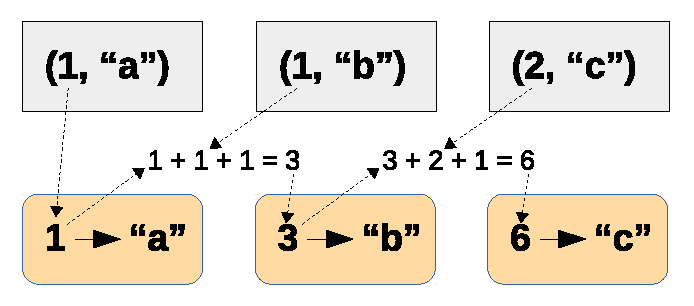
\includegraphics{figs/mech-2-very-short.eps}};
  \end{tikzpicture}
  \caption{An example delta dictionary.}
  %% \caption{What mapping is represented by the \dd~ $\dictP$?}
  \label{fig:dd-example}
\end{subfigure}
%% \end{figure}

\begin{figure}[b] %% [H]
  \centering
  \begin{tikzpicture}[nodes = {align = left}]
    \node [scale=.4]
    {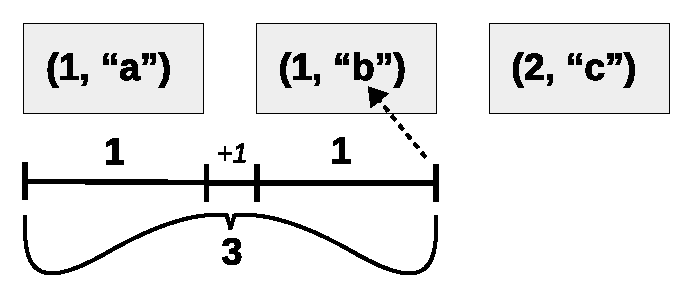
\includegraphics{figs/find-3-very-short.eps}};
  \end{tikzpicture}
  \caption{How do we find key $3$?} %% in the \dd?}
  \label{fig:dd-example-find}
\end{figure}

\begin{figure}[H]
  \centering
  \begin{tikzpicture}[nodes = {align = left}]
    \node [scale=.4]
    {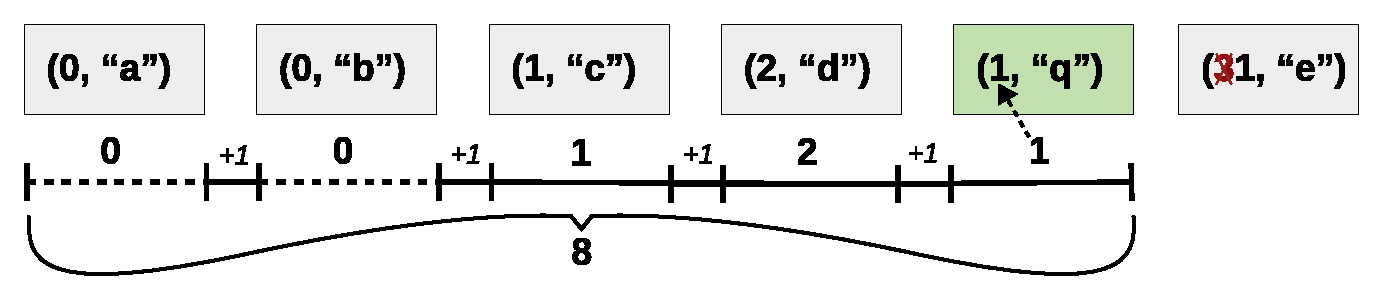
\includegraphics{figs/insert-8.eps}};
  \end{tikzpicture}
  \caption{How do we insert a mapping from key $8$ to value "q"?}
  \label{fig:find-6}
\end{figure}



%% \subsection{Bijections to the naturals}
%% \label{sec:DD:bij}
\parahead{Bijections to the naturals}
Note that the above definitions are in terms of a seemingly arbitrary key type,
and use a function \texttt{convert} to convert terms of that type into naturals.
In Agda, our \dd~ module accepts two parameters - the first is the key type \texttt{Key},
and the second is a type-class \texttt{bij}, whose three members are a \texttt{convert}
function that takes \texttt{Key}s to naturals, and proofs that \texttt{convert} is
injective and surjective. Thus, any key type can be used, as long as the developer
can define a function that converts it to a natural, and prove that that function is
bijective. As an example, we define a \texttt{bij} instance for integers. Other common
key types, such as other numeric types or strings, should be reasonably straightforward
to support. TODO further discussion about how this might be onerous for other key types,
like trees or ADTs. TODO discussion about how this won't work for finite types, like
characters, because we need a true bijection.

Although most types that are suitable for use as keys in the first place can be bijected to the
naturals, for some types defining this bijection may be too awkward or cumbersome, in which case {\dd}s may
be a poor choice.

\subsection{Lookup and Insertion}
\label{sec:DD:basics}
The basic functionality of dictionaries are lookup and insertion - they are defined as follows
(TODO):

\begin{figure*}
%% TODO using alltt temporarily, to inline DD.hs directly
\begin{alltt}
\input{code/DD.hs}
\end{alltt}
\caption{Delta dictionary implementation in Haskell.}
\label{fig:haskell}
\end{figure*}


The core theorems for lookup and insertion are as follows (TODO):

\subsection{Destruction}

\rkc{move a bunch of that material from Case Study to here}

\subsection{Additional Operations}

Our Agda mechanization also defines key deletion, union, map, and to/from-list operations, along
with appropriate metatheory (not reproduced here).



%% \subsection{Core properties}
\section{Properties}
\label{sec:DD:props}

\subsection{Design Goals}

The \SemInj~ and \EqDec~ theorems, a destruction theorem, and analogs to \emph{contraction} and
\emph{exchange} are defined below, and proven in Agda. \SemTot~ cannot be formally defined - rather
its truth is apparent from the fact that the other theorems do not require their \dd~ arguments to
be refined with validity premises.

\begin{proposition}[\SemTot]

\breakAndIndent
%
\rkc{Blah}

\end{proposition}

\begin{theorem}[\SemInj]
\label{thm:SemInj}

\breakAndIndent
%
For any {\dd}s $D_1$ and $D_2$,
%
if for all $k$, $D_1[k] = D_2[k]$,
%
then $D_1 = D_2$.

\end{theorem}

\begin{theorem}[\EqDec]
\label{thm:EqDec}

\breakAndIndent
%
For any {\dd}s $D_1$ and $D_2$ whose values are of type $V$,
%
given a function that decides equality for type $V$,
%

\justIndent
%
we can decide that either $D_1 = D_2$ or $D_1 \ne D_2$.

\end{theorem}

\begin{theorem}[\EzDstr]
\label{thm:EzDstr}

\breakAndIndent
%
For any \dd~ $D$,

\justIndent \quad
%
either $D = \emptyset$ OR

\justIndent \quad
%
there exist $D'$, $k \notin D'$, and $v$
%
s.t. $D = D' , (k, v)$.

\end{theorem}

\subsection{Contraction and Exchange}

\rkc{Two common properties for PL metatheory.}

\begin{theorem}[Dictionary Contraction]
\label{thm:cont-dicts}

\breakAndIndent
%
For any {\dd}~ $D$,
%
$D, (k, v'), (k, v) = D, (k, v)$.

\end{theorem}

\begin{theorem}[Dictionary Exchange]
\label{thm:exch-dicts}

\breakAndIndent
%
For any {\dd}~ $D$,
%
if $k_1 \ne k_2$, then
%
$D, (k_1, v_1), (k_2, v_2) = D, (k_2, v_2), (k_1, v_1)$.

\end{theorem}

%% \subsection{Practical Importance}
%% \label{sec:Problem:pract}
\section{Case Study}
\label{sec:CaseStudy}
To illustrate practical problems and solutions, we present a hypothetical case study of a developer working to
prove evaluation metatheory using environment-based semantics. This case study closely resembles the actual process we went
through on a real project, the difficulties of which created the necessity of inventing \dds. Of course,
because this case study involves a very particular situation, one which seems to be unusual (TODO sources?),
the problems we run into and solutions we suggest may not generalize. Accordingly, we use the case study to
present concrete illustrative examples, and follow each example with an argument of its applicability to more
general situations.

\newcommand{\eval}[3]{\ensuremath{{#1} \vdash {#2} \hspace{0.01in} \Rightarrow {#3}}}

At the outset, we have an evaluation judgment \eval{E}{e}{r}~ which takes an environment $E$ and an expression $e$
and "produces" a result $r$.
%Many mechanizations use substitution rather than environments, but (TODO source)
%explains why environment-based semantics are sometimes preferable. More generally, environments are only one use
%case for dictionaries, which are a very general purpose data structure that is likely to be used for a wide
%variety of other purposes.
$E$ is a finite map from variable names in scope to the results that are bound to
those variables. The question is "What data structure do we use to implement $E$?". The simple answer is a \sal,
and as long as we don't run into any problems on account of \SAL's lack of certain useful properties, the simple
answer is best.

But if we consider it important to prove the \emph{structural properties} \emph{contraction}
and \emph{exchange} (see \autoref{fig:con-exch}), we do run into a problem. These properties correspond,
respectively, to the irrelevance of duplication and reordering in the environment with regard to the judgment's
conclusions. The rule for lambda evaluation states that \mbox{\eval{E}{\lambda x . e}{[E]\lambda x . e}}, the result
being a closure over $E$. Using {\SAL}s, \mbox{\eval{E, (x, a), (x, b)}{\lambda x . e}{[E, (x, a), (x, b)]\lambda x . e}}
while \mbox{\eval{E, (x, b)}{\lambda x . e}{[E, (x, b)]\lambda x . e}}; $[E, (x, a), (x, b)]\lambda x . e \ne
[E, (x, b)]\lambda x . e$, so \emph{contraction} is violated. \emph{Exchange} is violated similarly. Many mechanizations
do not aim to prove \emph{contraction} and \emph{exchange} (TODO sources?), which makes our scenario somewhat
particular - however, they are two of the defining properties of structural logics, and as such are of critical
importance in many general cases (TODO source). Furthermore, inability to prove these theorems could be a red flag
of a bug in the judgment, so proving them has practical value, even if the judgment doesn't need to be strictly
structural.

%  \begin{figure}[H]
%    $
%    \inferrule*
%      {\eval{\lambda x . e}{}
%      {E, (x, b) \vdash T}
%    $
%    \caption{Evaluation rule for lambdas}
%    \label{fig:eval-lam}
%  \end{figure}

To address this problem, we need a data structure that possesses \SemInj. Since the semantics of dictionaries are
insensitive to duplication or ordering of insertions, the data structure must be likewise insensitive, so
that the language's equality primitive has the same meaning as semantic equality, and thus
\mbox{$E, (x, a), (x, b) = E, (x, b)$}. Note that proving \SemInj~ not only makes it possible to prove
\emph{contraction} and \emph{exchange}, but gives us these \emph{structural properties} essentially "for free".

  \begin{figure}[H]
    $
    \inferrule*[lab=\textbf{\large Contraction}]
      {\eval{E, (x, a), (x, b)}{e}{r}}
      {\eval{E, (x, b)}{e}{r}}
    $
    \quad\quad\quad\quad
    $
    \inferrule*[lab=\textbf{\large Exchange}]
      {\eval{E, (x, a), (y, b)}{e}{r} \\ x \ne y}
      {\eval{E, (y, b), (x, a)}{e}{r}}
    $
    \\\hfill\\\quad\quad
    $
      D, (x, a), (x, b) = D, (x, b)
    $
    \quad\quad
    $
      x \ne y \rightarrow D, (x, a), (y, b) = D, (y, b), (x, a)
    $
    \caption{Contraction and exchange theorems for \emph{eval}, as well as analogs for dictionary data structures that possess \SemInj (TODO source for contraction and exchange)}
    \label{fig:con-exch}
  \end{figure}

\newcommand{\refine}[2]{\ensuremath{{#1}\{\text{#2}\}}}

This problem can be addressed by switching from {\SAL}s to {\cal}s or {\fpf}s, because the latter two possess
\SemInj. Let's assume for the sake of discussion that we go with {\CAL}s. We run into another problem - {\CAL}s
do not possess \SemTot, because an arbitrary association list that type-checks may not be a valid \CAL.
An invalid association list can still be used in the same way a \SAL~ would, but we lose the
\SemInj~ property. Thus, wherever the \CAL~ goes, it must be refined with a proof of its validity. The ability
to refine ordinary types with proofs of validity is one of the most interesting and useful benefits of
dependently-typed languages, and this power should be appreciated. However, refining with proof terms can
come at a practical cost, so even in dependently-typed languages, there is high value in avoiding refinements
whenever possible (or at least whenever profitable). The practical cost of refinements is that proof terms
don't possess the properties \SemInj~ or \EqDec: due to \emph{proof relevance} (TODO source), two proofs of
the same property may be unequal, and due to the fact that proof terms may contain functions, the equality of
proof terms is not even decidable in the general case. With {\CAL}s, \mbox{$E, (x, a), (x, b) = E, (x, b)$},
but with refinements such as \refine{E}{proof\_of\_validity},
\mbox{$[\refine{(E, (x, a), (x, b))}{proof1}]\lambda x . e \ne [\refine{(E, (x, b))}{proof2}]\lambda x . e$},
so \emph{contraction} is once again violated. Perhaps we can work around this problem by moving the proof term
outside of the closure, to get \mbox{\refine{([E, (x, a), (x, b)]\lambda x . e)}{proof1}}, then defining a
special notion of equality for evaluation results, that treats closures specially by erasing the proof term
before checking equality with the built-in primitive, then definining \emph{contraction} and \emph{exchange}
in terms of this special notion of equality. However, this is all very cumbersome. We are no longer able to
use primitive equality when working with results, our special notion of equality should be decidable, but
not trivially so, and whenever we make any "modification" to an environment we must use theorems
to appropriately update the proof term and then repackage the new proof term with the new environment.
These sorts of pain points can crop up in any case where a refined object is being used as data, or must be
tested for equality with another refined object. Thus \SemTot, which obviates the need for refinement, has
a lot of practical value in many general cases.

{\FPF}s, sans refinement (TODO more discussion about the possibility of refinement?), do not technically
satisfy \SemTot, because a type-correct function may not
actually be finite. However, since we can't iterate, destruct, or query the size of {\FPF}s, the code
that works with dictionaries doesn't actually need to ensure that those dictionaries are finite. Lookup
and insertion will work just the same on finite and infinite partial functions, so there's generally no
practical need to refine them with proofs of finititude. Thus we can avoid the problems of validity refinement
by switching from {\CAL}s to {\FPF}s. But doing so creates new problems, since unlike the association lists,
{\FPF}s don't possess \EqDec. We can prove that
\mbox{$[E, (x, a), (x, b))]\lambda x . e = [E, (x, b)]\lambda x . e$}, and thus prove \emph{contraction} and
\emph{exchange}, but there's no way to determine whether two arbitrary results are equal or unequal.
The ability to decide equality has very general utility; in our particular case, we had an
\mbox{$\texttt{assert}~ e_1 = e_2$} form which would evaluate $e_1$ and $e_2$ and then check if the results
were equal, naturally requiring that equality of results be decidable. Additionally, as aforementioned,
it's not possible to iterate, destruct, or query the size of {\FPF}s, a critical limitation if there's
ever a need to inspect the environment or delete a mapping from it.

At this point it was necessary to invent a dictionary data structure that had all three critical properties:
\SemTot, \SemInj, and \EqDec. \EqDec~ ruled out function-based techniques, \SemInj~ required canonical
ordering and deduplication, and \SemTot~ meant that the canonical order and deduplication had to come from
how the data was interpreted rather than how it was organized. These requirements essentially defined the
mechanism of \dds. Of course, the non-literal way in which the data is interpreted means that it is not
safe for client code to work with the raw data directly, rather all interaction with the data must be
encapsulated in library functions. Unfortunately, this includes \emph{destruction}; an interaction which
normally goes through the very natural, elegant, and well-supported mechanism of pattern matching is now
only available through a library theorem:

\texttt{destruct-dd : (A : Type) (D : dd A) $\rightarrow \\
\phantom{xxxxxxxxxxxxxxxx} D = \emptyset \quad \lor \\
\phantom{xxxxxxxxxxxxxxxx} \exists~(n, a, D')~\left\{~ D = D' , (n, a) \quad \land \quad n \notin D' ~\right\}$}

Just as a list can be destructed with a case expression whose first branch matches nil and whose second branch
decomposes the list into a single item (particularly the head) and the remainder of the list, a \dd~ can be
destructed by matching the result of \texttt{destruct-dd} with a case expression whose left branch handles the
nil dictionary and whose right branch is provided a single item from the dictionary (the mapping $(n, a)$)
and the remainder of the dictionary ($D'$), as well as a proof that $D'$ really is $D$ minus the $(n, a)$
mapping.

This function achieves the same purpose as typical pattern matching (albeit more awkwardly), but because it
doesn't harness the primitive notions of pattern matching and structure, it doesn't establish structural
decrease on the dictionary object, which may break out-of-the-box structural recursion in the likely case
of recursion on $D'$. To enable manual establishment of structural recursion, via an extra parameter that
explicitly tracks the dictionary length, we provide another theorem:

\texttt{dd-extend-length : (A : Type) (D : dd A) (n : Nat) (a : A) $\rightarrow \\
\phantom{xxxxxxxxxxxxxxxxxxxxx} n \notin D \rightarrow \\
\phantom{xxxxxxxxxxxxxxxxxxxxx} |D, (n, a)| = 1 + |D|$}

Although possible, manually establishing termination is painful, especially given that it's not necessary
for {\SAL}s or {\CAL}s. Thus \dds~ fail at \EzDstr, although they are still better than {\FPF}s in this
regard, seeing as it's not only hard but impossible to destruct {\FPF}s. Is it possible to have a data
structure that possesses all four properties? Not likely - as mentioned above, the combination of
\SemInj~ and \SemTot~ essentially
necessitates that the data in the data structure be interpreted in a non-literal way, which in turn
makes it dangerous for client code to mess with the raw data. As such, we believe we've uncovered an
inherent trade-off between desirable properties. In our case, where \EqDec~ of results is critical,
and the need to destruct dictionaries is occasional but rare, \dds~ seem to be a clear winner over
{\CAL}s ({\SAL}s and {\FPF}s are unviable for our requirements), but in cases where dictionaries are
not used as data
(e.g. as a subcomponent of a closure) or at least not data that needs to be tested with equality, and
where dictionaries sometimes need to be inspected or destructed, {\CAL}s may be a preferable.

\section{Discussion and Related Work}
\label{sec:Discussion}

\vspace{0.05in} %% SPACE HACK

%% \parahead{Association Lists and Partial Functions}
%% \parahead{Conventional Dictionary Representations}

\parahead{Conventional Representations}
%
Due to their simplicity, {\sal}s are perhaps the most typical implementation for dictionaries.
%
But because \SemInj{} is so important in simplifying proofs, {\FPF}s also see significant use---in key works such as \emph{Software Foundations}~\cite[Maps]{Pierce:SF1}---despite requiring a bit of extra overhead.

%% TODO macro?

\Cals{} seem to get little use, perhaps because working with refinement proofs might add more hassle than \SemInj{} alleviates.
%
\Cals{} are defined in the Coq standard library as \texttt{FMapList} \citep{FMapList}; a GitHub search for \texttt{FMapList} shows $304$ results,
%
whereas a search for \texttt{FMapAVL} shows $474$ results, suggesting that {\cal}s have been found to be less useful than high-performance implementations.
%
A search for \texttt{FunctionalExtensionality} \citep{FunExt}, on the other hand, turns up $4916$ results, though most of these are probably unrelated to dictionaries.
\footnote{
%
These searches and can be reproduced by URLs of the form:
\url{https://github.com/search?l=\&p=3\&q=FMapList+language\%3ACoq\&ref=advsearch\&type=Code },
replacing \texttt{FMapList} with \texttt{FMapAVL} and \texttt{FunctionalExtensionality}.
%
Accessed August 23, 2020.
%
}
%
\citet{Amorim:fmap} provides a more comprehensive treatment of {\cal}s, augmenting them with a functional interface so that the client can
%
use them as though they were {\fpf}s (note that this is different from having a \fpf{} augmented with keys).

% github searches
% funext        : 4916
% FMapInterface : 504
% FMapAVL       : 474
% FMapList      : 304

\parahead{Dictionaries vs. Custom Datatypes}

Dictionaries are not always used to represent environments in mechanizations of programming language theory.

When the order of bindings does not matter, dictionaries are a natural choice for type contexts.
%
But if types defined ``later,'' or in inner scopes, can refer to types defined ``earlier,'' or in outer scopes, then order-insensitive dictionaries are inherently inappropriate.
%
This is the case for languages that support subtyping (notably, the subject of the POPLMark challenge~\citep{XXX}).
%
Linear logics, on the other hand, require sensitivity to duplicate insertions, so duplication-insensitive dictionaries are inappropriate for them as well.
%
Though {\sal}s remain the most natural choice in these cases, future work could explore data structures that are sensitive to ordering but not duplication, or vice versa.

The use of dictionaries is furthermore avoided in many systems that use substitution rather than environments
%
in defining the dynamic semantics of a language, as well as the many systems that avoid named variables altogether by using De Bruijn indices \cite{XXX,XXX,XXX} or comparable techniques.

For these reasons, many existing mechanizations make little use of order-and-duplication-insensitive dictionaries. 
%
However, as mechanization becomes increasingly popular, for an ever-broadening scope of applications,
%
it seems inevitable that a programming utility as fundamental as dictionaries will eventually become ubiquitous, at which point it will be important to have the
%
best implementations at our disposal.

\parahead{Performance Concerns}
%
It was noted above that AVL implementations are apparently more popular than {\cal}s, and as more software is mechanized, performance is likely to become an
%
even greater concern than it is today. In cases where there is no extraction step, and the proof language is also the language that will be executed,
%
there may be no choice but to use implementations that are high-performance but theoretically unwieldy. However, it seems more appropriate, especially with
%
fundamental utilities such as dictionaries, to either extract or transpile the mechanization into an implementation language that defines these utilities natively
%
by way of highly efficient implementations such as hashtables or red-black trees. This extraction may not be completely fidelitous, since it will be using a
%
different data structure in the implementation than was used in the proofs, but presumably the implementation's version of dictionaries is well-tested and bug-free,
%
and its definition of equality is, at least for fundamental utilities such as dictionaries, extensional and decidable. Regardless, even if unperformant implementations
%
cannot be used for code that will be run, they may be useful for parts of the code which are only used for proofs and will not be executed.

\parahead{Future Work}
%
This paper discusses the important properties \SemTot, \SemInj, \EqDec, and \EzDstr, and offers an implementation for dictionaries that (mostly) fulfills these properties.
%
Future work could consider implementations for other key utilities, such as trees or graphs, that satisfy these properties.
%
Doing so could be far more challenging.
%
It is relatively easy to simultaneously satisfy \SemTot{} and \SemInj{} for list-like structures such as dictionaries,
%
but much more awkward to do so for highly structural data such as graphs. For unlabeled graphs in particular, establishing a one-to-one correspondence between terms and
%
semantic meanings requires understanding of the graph isomorphism problem, which involves complex algebra.

% Other things to consider mentioning, but probably not
% - try to make sense of https://github.com/arthuraa/coq-utils/blob/master/theories/nominal.v
% - Coq also has FMapPositive, which is a tree based on the binary representation
% - something something explicit substitutions, Abadi et al. POPL 1990.
% - Look deeper into TDD with Idris


%% \begin{acks}
%% To Robert, for the bagels and explaining CMYK and color spaces.
%% \end{acks}

\bibliographystyle{ACM-Reference-Format}
\bibliography{references}

%% \appendix

\end{document}
\endinput
